\documentclass[english,a4paper]{report}
%%%%%%%%%%%%%%%%%%%%%%%%%%%%%%%%%%%%%%%%%%%%%%%%%%%%%%%%%%%%%%%%%%%%%%%%%%%%%%%%%%%%%%%%%%%%%%%%%%%%%%%%%%%%%%%%%%
\usepackage{babel}
\usepackage{hyperref}
\usepackage{t1enc}
%\usepackage{aeguill}
\usepackage{varioref}
\usepackage{fancyvrb}
\usepackage{color}
\usepackage{cite}
\usepackage{graphicx}
\usepackage{float}
\usepackage{listings}
\usepackage{harvard}
\usepackage{geometry}
\usepackage{graphics}
\usepackage{setspace}
\usepackage{thumbpdf}
\usepackage{fancyhdr}
\usepackage{lastpage}
\usepackage{alltt}
\usepackage{graphicx}
\usepackage{verbatim}
\usepackage{color}
\usepackage{url}
\usepackage{epsf}
\usepackage{listings}
\usepackage[refpages]{gloss}
\usepackage{array}
\usepackage{longtable}
\usepackage{multirow}
\usepackage{amsmath, amsthm, amssymb}
\usepackage{slashbox}
\usepackage{rotating}
%%%%%%%%%%%%%%%%%%%%%%%%%%%%%%%%%%%%%%%%%%%%%%%%%%%%%%%%%%%%%%%%%%%%%%%%%%%%%%%%%%%%%%%%%%%%%%%%%%%%%%%%%%%%%%%%%%

\geometry{verbose,a4paper,tmargin=30mm,bmargin=30mm,lmargin=30mm,rmargin=30mm}

\pagestyle{fancy}
\fancyhf{}
\renewcommand{\sectionmark}[1]{\markboth{ \thesection.\ \emph{#1}}{}}
\renewcommand{\chaptermark}[1]{\markboth{ \thechapter.\ \emph{#1}}{}}

\fancyhead[RO]{\leftmark}

\fancyhead[LE]{\small{\it Visual Languages}}

\fancyfoot[CE,CO]{\thepage}
\lstset{basicstyle=\small,
numbers=left, numberstyle=\tiny, numbersep=5pt,
breaklines=true, mathescape=true, frame=tB}


%%%%%%%%%%%%%%%%%%%%%%%%%%%%%%%%%%%%%%%%%%%%%%%%%%%%%%%%%%%%%%%%%%%%%%%%%%%%%%%%%%%%%%%%%%%%%%%%%%%%%%%%%%%%%%%%%%
\begin{document}
\begin{titlepage}
\thispagestyle{empty}
\begin{figure}[htbp]
\begin{center}

\includegraphics[width=0.3\textwidth]{Images/DI-UM}
\end{center}
\end{figure}
{\centering \large
{\large\bf \textbf{Universidade do Minho} \\ Departamento de Inform�tica}\\
\vspace{1cm}
\bf{Engenharia de Linguagens}\\
\vspace{2cm}
{\Large \bf {Projecto Integrado}}\\
\vspace{1cm}
{\LARGE \bf {\emph{Software} para An�lise e Avalia��o de Programas}}\\
\vspace{1cm}
%{\large \bf {}}
\vspace{8.5cm}
}
\flushleft{ \emph{Grupo 2:\\}
\vspace{0.4cm}
Jos� Pedro Silva\\
M�rio Ulisses Costa\\
Pedro Faria\\
}
\vspace {1.5cm}
\textbf{Braga, \today}\\
\pagebreak
\end{titlepage}

\thispagestyle{plain}
\chapter*{Abstract}

Este relatório trata da primeira fase do Projecto Integrado (PI) da UCE de Engenharia de Linguagens. O PI consiste num sistema
de sbmissão de trabalhos dos alunos. Este sistema deve ser capaz de aceitar registos de alunos e professores. Deve ainda permitir a submissão
de código por parte dos alunos e a submissão de exercicios por parte dos professores. O sistema deve ainda ser capaz de fazer uma análise detalhada
sobre o código submetido pelo aluno e gerar um relatório para o professor ler sobre este mesmo código.\\

Nesta fase o grande objectivo é modelar todo este sistema, decidimos fazê-lo de um ponto de mais técnico, com alguns diagramas e estrutura dos ficheiros XML que vão
ser úteis para a nossa implementação, mas também decidiu-se fazer uma modelação do ponto de vista mais formal, de forma a nesta fase clarificar o processo de
modelação e fazer com que dêmos maior foco à modelação em si. Semt er de pensar nos sistemas complexos qe estão por trás disso.



\tableofcontents
\listoffigures
\listoftables
\newpage


\pagenumbering{arabic}
\newpage
%%%%%%%%%%%%%%%%%%%%%%%%%%%%%%%%%%%%%%%%%%%%%%%%%%%%%%%%%%%%%%%%%%%%%%%%%%%%%%%%%%%%%%%%%%%%%%%%%%%%%%%%%%%%%%%%%%
\chapter{Introdu��o} \label{chap int}
Contextualiza��o do cap 2... 

\section{Motiva��o}
Motiva��o...
\section{Objectivos}
Este projecto tem como objectivos consolidar conhecimentos adquiridos nos diferentes m�dulos da UCE de Engenharia de Linguagens. Para isso, o \emph{software} pretendido 

\section{Estrutura do Relat�rio}
Estrutura do Relatório...


\newpage
%%%%%%%%%%%%%%%%%%%%%%%%%%%%%%%%%%%%%%%%%%%%%%%%%%%%%%%%%%%%%%%%%%%%%%%%%%%%%%%%%%%%%%%%%%%%%%%%%%%%%%%%%%%%%%%%%%
\chapter{Chapter2} \label{chap xxx}
Contextualiza��o do cap 2... 

\section{Sec2}
Sec 2\label{sec yyy}
\newpage
%%%%%%%%%%%%%%%%%%%%%%%%%%%%%%%%%%%%%%%%%%%%%%%%%%%%%%%%%%%%%%%%%%%%%%%%%%%%%%%%%%%%%%%%%%%%%%%%%%%%%%%%%%%%%%%%%%
\chapter{Modela��o do Problema} \label{chap modprob}
Contextualiza��o do cap 2... 

\section{Modela��o Informal}
Com o diagrama da arquitectura do sistema, figura~\ref{fig diaact},pretende-se mostrar as várias entidades que podem aceder ao sistema, assim como as várias
actividades que cada uma pode realizar e tarefas para o sistema processar.
Também é realçada a ideia de que alguns dos recursos do sistema só estão dispóniveis ao utilizador depois 
de passar por outros passos, ou seja, o diagrama dá a entender a ordem pelas quais o utilizador e o sistema podem/devem executar as tarefas.\\

\begin{figure}[htbp]
\begin{center}
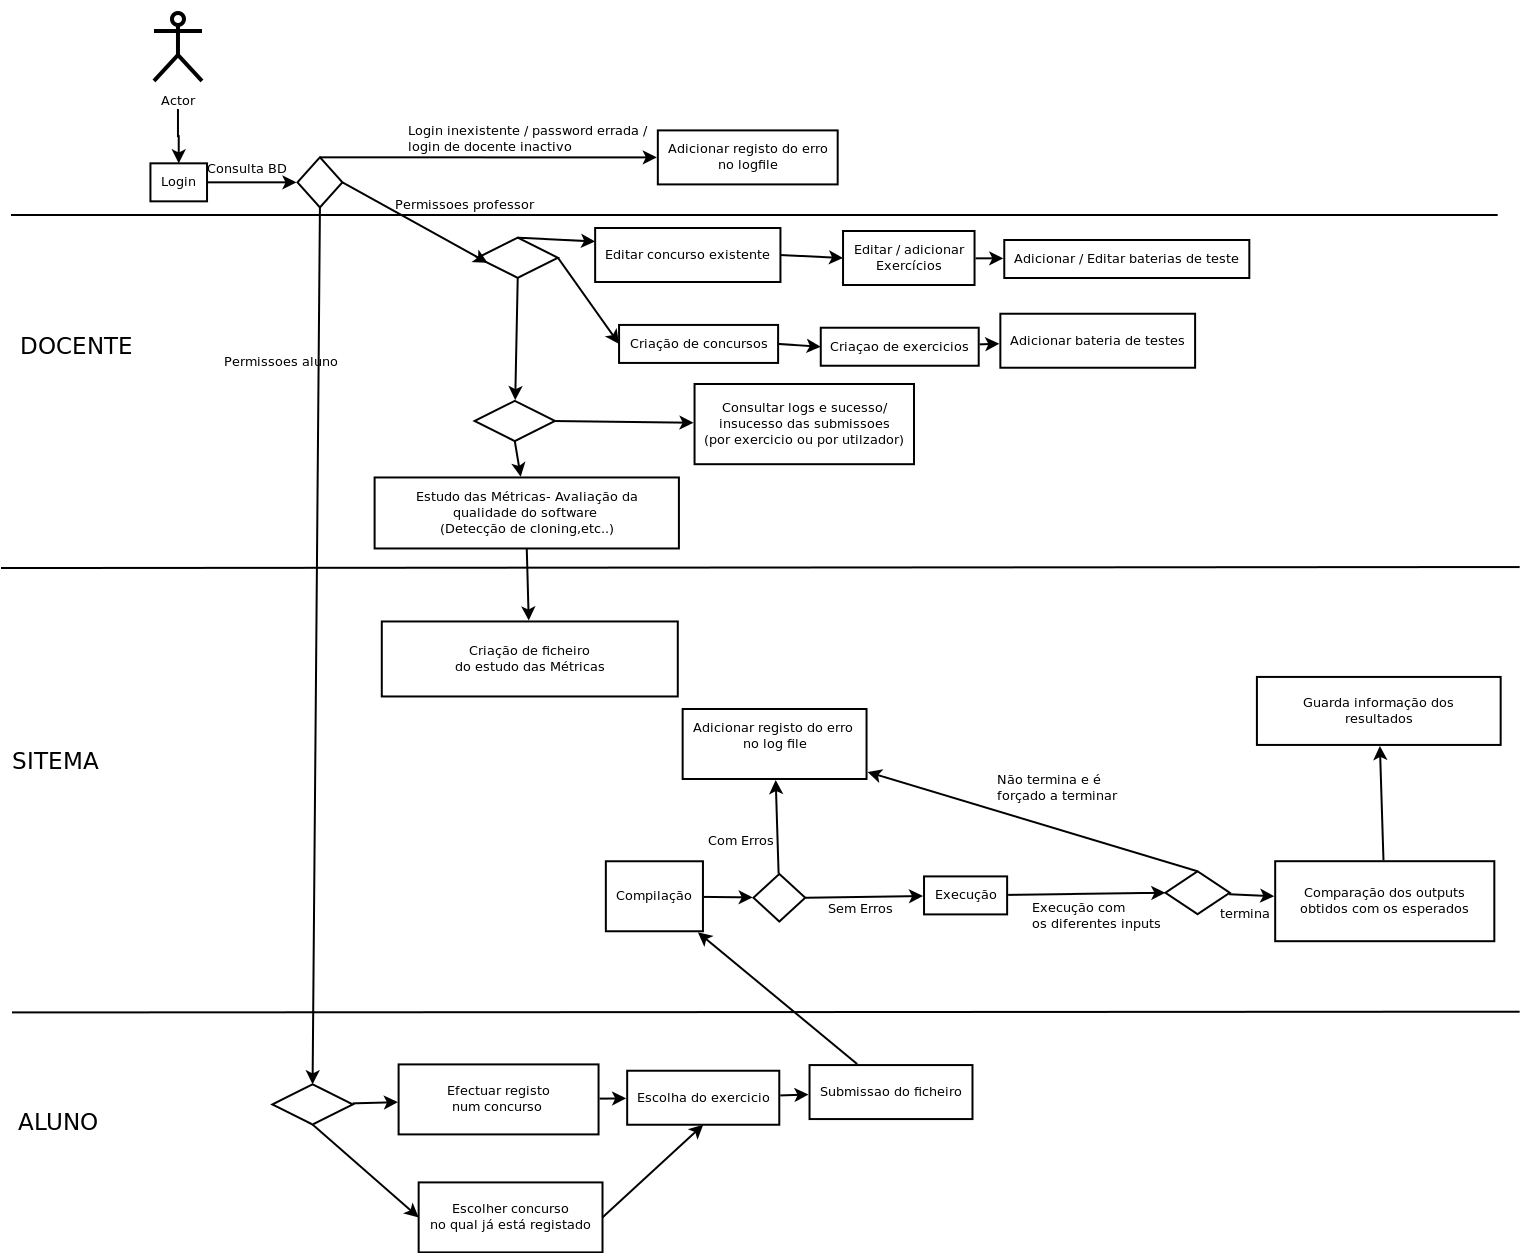
\includegraphics[width=0.5\textwidth]{Images/EL-PI}
\caption{Diagrama de actividades::notanotanota}\label{fig diaact}
\end{center}
\end{figure}

Para começar, como temos duas entidades diferentes que podem aceder ao sistema (o docente e o aluno/concorrente), 
dividiu-se o diagrama em duas partes distintas (uma para cada entidade referida), de modo a facilitar a leitura.\\

Em ambos os casos, o login é a primeira actividade que pode ser realizada.
Se o login não foi efectuado com sucesso, é adicionado no log file uma entrada com a descrição do erro.
No caso de o login ser efectuado com sucesso, consoante as permissões do utilizador em questão, tem diferentes opções ao seu dispôr.\\

No caso do login pertencer a um docente, este terá acesso aos dados de cada um dos grupos, podendo verificar os resultados que estes 
obtiveram na resolução das questões do(s) concurso(s), assim como ao ficheiro que contém a análise das métricas dos vários programas submetidos 
pelos mesmos.
Poderá também criar novos concursos e os seus respectivos exercícios, assim como adicionar baterias de testes para os novos exercícios, 
ou para exercícios já existentes.\\

No caso do login pertencer a um aluno/concorrente, o utilizador terá a opção de se registar num concurso ou de seleccionar um no qual já 
esteja registado.
Já depois de seleccionar o concurso, pode ainda escolher o exercício que pretende submeter.
Depois de submeter o código fonte do programa correspondente ao exercício escolhido, e já sem a interacção do utilizador, 
o sistema compilará e tentará executar os diferentes inputs da bateria de testes do exercício, e compararar os resultados obtidos com os esperados.
No fim de cada um destes procedimentos, serão guardados os resultados / erros.
Para terminar, será feito um estudo das métricas do ficheiro submetido, tendo como resultado a criação um ficheiro com os dados relativos a essa avaliação.\\
\label{sec modinf}
\section{Modela��o Formal}
Contextualiza��o do cap 2... 
\label{sec modfor}
\section{Modela��o � l� cenas}
--estas metricas sao importantes para model driven arquitecture ?
Este conjunto de métricas são referidas em vários papers e sem sombra de dúvidas são as mais estudas, também as mais utilizadas para avaliar modelos UML.
Estas focam-se mais nos diagramas de classes visto estes serem os que mais facilmente se transformam em código e é preciso ter
em consideração que como estas regras derivam directamente do modelo OO, é mais fácil aplica-las
aos diagramas de classes. Para além disso este tipo de diagrams do ponto de vista da implementação dão uma visão mais geral do sistema que modela.
Estas métricas em particular são detalhadas por McQuillan e Power em ~\cite{Power}. Existe também um software ~\cite{SDMetrics}(SDMetrics) que avalia além destas, um conjunto mais extenso de métricas, que analisa outros diagramas além do de classes, como por exemplo os diagramas de estados e de actividades.

\label{sec modcenas}
\section{Modelo de Dados}
Definiu-se que existir�o tr�s tipos de utilizadores: o administrador, o docente e o aluno/concorrente.\\

\begin{itemize}
  \item Administrador - � a entidade com mais poder no sistema. � o �nico que pode criar contas do tipo docente. � caracterizado por:
    \begin{itemize}
      \item Nome de utilizador;
      \item Nome completo;
      \item Password
      \item e-Mail
    \end{itemize}
  \item Docente - entidade que tem permiss�es para criar concursos, exerc�cios, aceder aos resultados das submiss�es, (...). Os seus atributos coincidem com os do Administrador.
  \item Aluno/Concorrente - (...)
\end{itemize}

Decidiu-se que o sistema ter� a no��o de grupo. 
(...)
O grupo � que possui as credenciais para entrar no sistema (nome de utilizador e password). 
Al�m disso tamb�m tem um nome pelo qual � identificado, um e-mail que ser� usado no caso de haver necessidade de se entrar em contacto com o grupo, e um conjunto de concorrentes.\\

\begin{figure}[htbp]
\begin{center}

\includegraphics[width=0.5\textwidth]{Images/missimage}
\caption{Modelo de dados}\label{fig modedados}
\end{center}
\end{figure}

Achamos importante incluir a informa��o de cada concorrente no grupo para, se poss�vel, automatizar v�rias tarefas tais como lan�amento de notas.
Cada concorrente � caracterizado pelo seu nome completo, n�mero de aluno (se for o caso), e e-mail.\\

Para finalizar vamos explicar em que consistem os concursos, exerc�cios e tentativas.

Um concurso, resumidamente, � um agregado de enunciados. 
Tem outras propriedades tais como um t�tulo, data de inicio e data de fim (per�odo em que o concurso est� dispon�vel para que os grupos se registem), 
chave de acesso (necess�ria para o registo dos grupos), dura��o do concurso (tempo que o grupo tem para resolver os exerc�cios do concurso, 
a partir do momento que d� inicio � prova), e por fim, regras de classifica��o.\\

Um enunciado � um exerc�cio que o concorrente tenta solucionar. Como seria de esperar, cada exerc�cio pode ter uma cota��o diferente, 
logo o peso do enunciado � guardado no mesmo. 
Para cada enunciado existe tamb�m um conjunto de inputs e outputs, que servir�o para verificar se o programa submetido est� correcto. 
Cont�m ainda uma descri��o do problema que o concorrente deve resolver, assim como uma fun��o de avalia��o, fun��o esta que define como se verifica se o output obtido est� de acordo com o esperado.\\
\label{sec modedados}
\newpage
%%%%%%%%%%%%%%%%%%%%%%%%%%%%%%%%%%%%%%%%%%%%%%%%%%%%%%%%%%%%%%%%%%%%%%%%%%%%%%%%%%%%%%%%%%%%%%%%%%%%%%%%%%%%%%%%%%
\chapter{Conclus�o e Trabalho Futuro}\label{chap con} 
Contextualiza��o...
\newpage
%%%%%%%%%%%%%%%%%%%%%%%%%%%%%%%%%%%%%%%%%%%%%%%%%%%%%%%%%%%%%%%%%%%%%%%%%%%%%%%%%%%%%%%%%%%%%%%%%%%%%%%%%%%%%%%%%%
\bibliographystyle{harvard}
%\bibliographystyle{plain}
\bibliography{bib}
\end{document} 
